\documentclass{beamer}

\usepackage[utf8]{inputenc}
\usepackage[portuguese]{babel}
\usepackage{graphicx}
\graphicspath{ {./images/} }
\usetheme{CambridgeUS}

\title{Questões 1-4 de forma didática}
\subtitle{Cálculo para Computação}
\author{Luiz Glomyer, Luiz Osmar, Christian Cruz, Farley}
\institute{Escola Superior de Tecnologia - UEA}
\date{\today}


\begin{document}

	\begin{frame}
		\titlepage
	\end{frame}
	
	\section{Primeira Questão}
	\subsection{Cálculo para Computação}
	\begin{frame}
		1) Um investidor aplica na bolsa de valores determinada quantia que triplica em 30 meses. Em quanto tempo essa quantia será quadruplicada, supondo-se que o aumento é proporcional ao investimento feito?
		
		\begin{figure}
			\centering
			
\includegraphics[]{Investidor-1.jpg}
			\label{fig:investidor-1}
		\end{figure}
	\end{frame}

	\begin{frame}{Modelando o problema}
		Para modelar, ou seja, transformar o nosso problema na linguagem matemática, faremos as seguintes convenções:
		\newline
		\pause
		
		\begin{itemize}
			\item  mediremos o tempo em meses e o chamaremos de t
			\item a quantia em um determinado instante de tempo será chamada de y
			\item chamaremos o investimento feito em uma certa quantidade de meses de y\textsubscript{0} (investimento inicial)
		\end{itemize}
	
		\begin{figure}
			\centering
			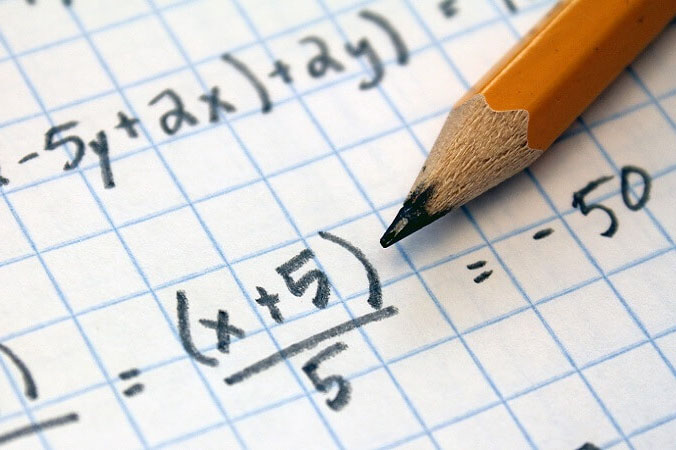
\includegraphics[scale=0.2]{matematica.jpg}
			\label{}
		\end{figure}
	\end{frame}

		\begin{frame}
		Devemos achar o tempo necessário até que a quantia investida se quadruplique, ou seja, o valor de t para a quantia 4y\textsubscript{0}. Temos, portanto:
		
		 \begin{displaymath}
		 \frac{dy}{dt} = Ky
		 \end{displaymath} \pause
		 
		 \begin{displaymath}
		 	 \frac{dy}{y} = K dt
		 \end{displaymath} \pause
		 
		 \begin{displaymath}
		 \int \frac{dy}{y} = \int K dt
		 \end{displaymath} \pause
		 
		 \begin{displaymath}
		 	\ln y = Kt + C
		 \end{displaymath} \pause
		 
		 Mas como C é uma constante arbitrária (pode assumir qualquer valor), podemos fazer \(C = \ln C_{1}\)
	\end{frame}
	
	\begin{frame}
		Substituindo a constante C e usando as propriedades de logaritmos: 
		\begin{displaymath}
			\ln y = Kt + \ln C_{1}
		\end{displaymath} \pause
		
		\begin{displaymath}
			Kt = \ln \frac{y}{C_{1}}
		\end{displaymath} \pause
		
		\begin{displaymath}
			\frac{y}{C_{1}} = e^{Kt}
		\end{displaymath} \pause
		
		
		Chegando, finalmente, na equação
		\begin{equation}
			\boxed{ y = C_{1}e^{Kt} }
		\end{equation}	
	\end{frame}
	
	\begin{frame}
		O investimento inicial é dado por y\textsubscript{0}, no tempo t = 0. Substituindo na equação (1):
		
		\begin{displaymath}
		y_{0} = C_{1}e^0 \therefore	C_{1} = y_{0}
		\end{displaymath} \pause
		
		Substituindo o valor de C\textsubscript{1} na equação (1):
		
		\begin{equation}
			\boxed{ y = y_{0}e^{Kt} }
		\end{equation}
		
		Obtemos então nossa equação geral. Como o valor investido na bolsa de valores triplica em 30 meses, fazemos \(y = 3y_0\) (triplicando o investimento inicial) e \(t = 30\) (30 meses) e substituímos os valores na equação (2):
	\end{frame}

	\begin{frame}
		\begin{displaymath}
			3y_0 = y_0e^{30K} \therefore 3 = e^{30K} 
		\end{displaymath} \pause
		
		Para descobrir o tempo até que a quantia seja quadruplicada, fazemos \(y = 4y_0\) na equação (2):
		
		\begin{displaymath}
 			4y_0 = y_0e^{Kt} \therefore 4 = e^{Kt} 
		\end{displaymath} \pause
		
		Mas, das duas equações acima, temos que: \( 4^{30} = e^{30Kt} \) e \( 3^t = e^{30Kt} \). Portanto:

		\begin{displaymath}
			4^{30} = 3^t \implies 30\ln 4 = t\ln 3
		\end{displaymath}
	\end{frame}

	\begin{frame}
		\begin{displaymath}
			t = 30 \frac{\ln 4}{\ln 3} \therefore t = 37,8 \text{ meses}
		\end{displaymath}
		
		Ou seja, o tempo necessário até que a quantia se quadruplique é de 37 meses e 24 dias
		
		\begin{figure}
			\centering
			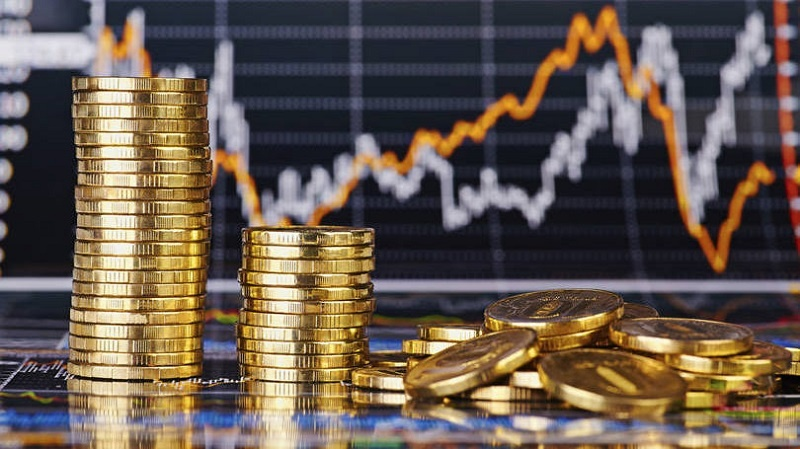
\includegraphics[scale=0.3]{dinheiro.jpg}
			\label{}
		\end{figure}
	\end{frame}
	\setcounter{equation}{0}
	
	\section{Segunda Questão}
	\subsection{Cálculo para Computação}
	\begin{frame}
		2) De um ponto situado a 120 m do solo joga-se uma pedra de massa 0,5 kg para o alto com uma velocidade inicial de 8 m/s. Desprezando-se a resistência do ar e quaisquer outras forças que porventura atuem sobre a pedra, à exceção da gravidade (10 m/s\textsuperscript{2}), calcular o tempo, a velocidade, e o espaço percorrido pela pedra até esta tocar o solo.
		
		\begin{figure}
			\centering
			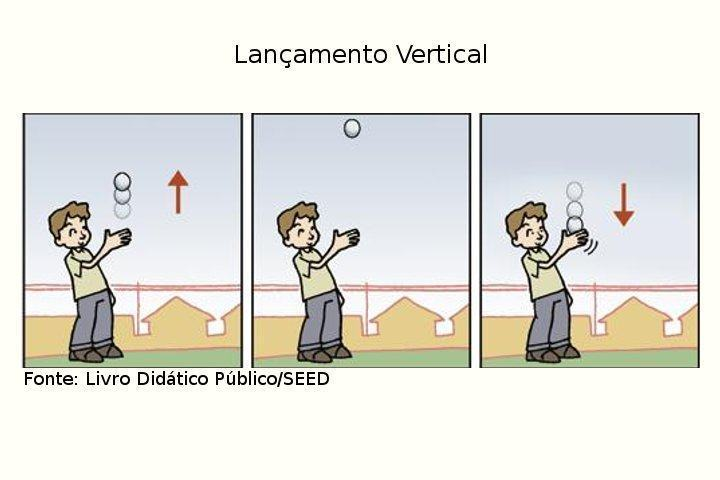
\includegraphics[scale=0.4]{lancamento.jpg}
			\label{}
		\end{figure}
	\end{frame}

	\begin{frame}
		Tomamos o nosso referencial (origem) na superfície da Terra, local onde a pedra foi arremessada.
		\begin{figure}
			\centering
			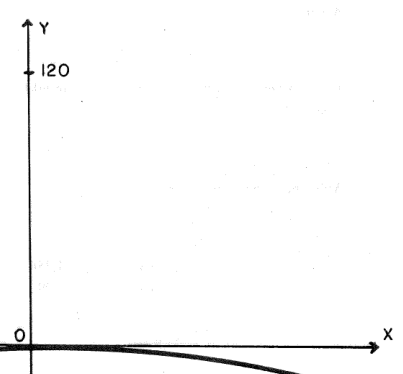
\includegraphics[scale=0.4]{eixo.png}
			\label{}
		\end{figure}
		
		Temos que \(F = ma = mg\), mas como o peso atua no sentido contrário ao movimento, temos que \(F = -mg\). Devemos ainda notar que a velocidade terá valores positivos na subida e negativos na descida.
	\end{frame}
	 
	\begin{frame}
		Como a aceleração é a derivada da velocidade em relação ao tempo e g = 10, temos que: \pause
		
		\begin{displaymath}
			m\frac{dv}{dt} = -mg
		\end{displaymath}
		
		\begin{displaymath}
			\frac{dv}{dt} = -10 \therefore dv = -10 dt 
		\end{displaymath}
		
		\begin{equation}
			v = -10t + C_1
		\end{equation} \pause
		
		No tempo t = 0 a velocidade inicial é 8 m/s. Substituindo na equação (1):
		
		\begin{displaymath}
			8 = -10(0) + C_1 \therefore C_1= 8
		\end{displaymath} \pause
		
		De posse do valor da constante C\textsubscript{1} e aplicando-o na equação (1), obtemos a seguinte equação:
		
		\begin{equation}
			\boxed{ v = -10t + 8}
		\end{equation}
	\end{frame}
	
	\begin{frame}
		Mas como a velocidade é a derivada do espaço percorrido em relação ao tempo, isso nos leva a:
		
		\begin{displaymath}
			\frac{dy}{dt} =-10t + 8
		\end{displaymath}
		
		\begin{displaymath}
			\int dy = \int (-10t +8) dy \therefore y = \frac{-10t^2}{2} + 8t + C_2
		\end{displaymath} \pause
		
		Quando t = 0 e y = 120 tem-se que \(C_2 = 120\). Assim:
		
		\begin{equation}
			\boxed{ y = -5t^2 +8t + 120 }
		\end{equation} \pause
		
		A pedra chega ao solo em y = 0, então:
		
		\begin{displaymath}
			5t^2 - 8t - 120 = 0
		\end{displaymath}
	\end{frame}
	
	\begin{frame}
		Resolvendo a equação de segundo grau obtemos os valores possíveis de t:
		
		$$\left\{ \begin{array}{l}
		t = 5,7\\
		t = -4,1\\
		\end{array}
		\right.$$ \pause
		
		Para se obter a velocidade no instante que a pedra toca o chão usamos o valor positivo de t na equação (2): 
		
		\begin{displaymath}
			v = -10(5,7) + 8 \therefore v = -49 \text{ m/s}
		\end{displaymath} \pause
		
		Na altura máxima a velocidade da pedra é igual a 0, ou seja, v = 0. Usando a equação (2):
		
		\begin{displaymath}
			0 = -10t + 8 \therefore t = 0,8 \text{ segundos}
		\end{displaymath} \pause
		
		Que é o tempo para a pedra chegar a 120 m. Como v = v\textsubscript{0} - gt e v = \(\frac{dy}{dt}\), tem-se: \(\frac{dy}{dt} = 8 - 10t\)
		
		
	\end{frame}
	
	\begin{frame}
		
		Integrando:
		
		\begin{displaymath}
			\int dy = \int (8 - 10t) dt \therefore  y = -5t^2 +8t + C
		\end{displaymath}
		
		Tomando C = 0 como referencial, temos que y = 3,20 m, ou seja, a distância do lançamento até a altura máxima. A distância total percorrida será:
		
		\begin{displaymath}
			3,2 + 3,2 + 120 = \boxed{ 126,4 \text{ m} }
		\end{displaymath}
		
		\begin{figure}
			\centering
			
\includegraphics[scale=0.25]{newton.jpg}
			\label{}
		\end{figure}
		
	\end{frame}
	\setcounter{equation}{0}
	
	\section{Terceira Questão}
	\subsection{Cálculo para Computação}
	\begin{frame}
		3) Em um depósito há 100 L de uma solução aquosa que contém 10 kg de sal. Joga-se água neste depósito com uma velocidade de 3 L/min ao mesmo tempo que, através de um orifício desse tanque, a mistura se escoa com uma velocidade de 2 L/min. A mistura se mantém homogênea mexendo-se a água com um agitador. Que quantidade de sal haverá no tanque 1 h depois de iniciada a operação?
		
		\begin{figure}
			\centering
			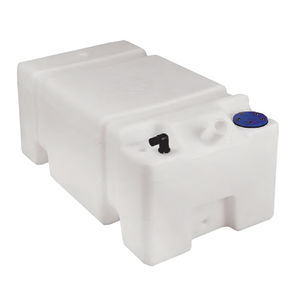
\includegraphics[scale=0.5]{tanque.jpg}
			\label{}
		\end{figure}
	\end{frame}
	\setcounter{equation}{0}

	\begin{frame}
		Definiremos
		\begin{itemize}
			\item y como o peso de sal escoado em kg \pause
			\item v como o volume \pause
			\item t como o tempo decorrido em minutos \pause
			\item \(\frac{dv}{dt}\) como a vasão (volume escoado por unidade de tempo) \pause
			\item \(\frac{dy}{dv}\) como a concentração, ou seja, a quantidade de sal por unidade de volume \pause
		\end{itemize}
		A taxa de escoamento do sal será:
		
		\begin{displaymath}
			\frac{dy}{dt} = \frac{dy}{dv} \frac{dv}{dt}
		\end{displaymath} \pause
		
		A concentração em cada instante será dada por:
		
		\begin{displaymath}
			\frac{dy}{dv} = \frac{10 - y}{100 + t}
		\end{displaymath}
	\end{frame}

	\begin{frame}
		Ou seja, pela razão entre o peso inicial de sal menos o peso escoado e o volume igual ao inicial (100 L) mais o adicionado (\(\int^v_0 dv= 3\int^t_0 dt\)) menos o escoado (\(\int^v_0 dv= 2\int^t_0 dt\))
		
		Assim:
		
		\begin{displaymath}
			100 + 3 \int^t_0 dt - 2 \int^t_0 dt = 100 + t
		\end{displaymath} \pause
		
		Logo:
		
		\begin{displaymath}
			\frac{dy}{dt} = 2 \frac{10 - y} {100 + t} \therefore \frac{dy}{10 - y} = 2 \frac{dt}{100 + t}
		\end{displaymath} \pause
		
		Integrando a igualdade acima, obtemos:
		
		\begin{displaymath}
			-\ln(10-y) = 2 \ln(100 + t) + C
		\end{displaymath}
	\end{frame}
	
	\begin{frame}
		Pelas condições iniciais, t = 0 e y = 0 (nenhuma quantidade de sal escoada), determina-se C
		
		\begin{displaymath}
			-\ln 10 = 2 \ln 100 + C \therefore C = -5 \ln 10
		\end{displaymath} \pause
		
		Então:
		
		\begin{displaymath}
			-\ln(10 - y) = 2\ln(100 + t) - 5\ln 10
		\end{displaymath}\pause
		
		\begin{displaymath}
			\ln(10 - y) = 5\ln 10 - 2\ln(100 + t)
		\end{displaymath} \pause	
		
		\begin{displaymath}
		10 - y = e^{5\ln10} \cdot e^{-2\ln(100 + t)}
		\end{displaymath} \pause
		
		\begin{displaymath}
		10 - y = e^{ln(10^5)} \cdot e^{\ln(100 + t)^-2}
		\end{displaymath}
	\end{frame}
	
	\begin{frame}
		Simplificando:
		
		\begin{displaymath}
			10 - y = 10^5 \cdot (100 + t)^-2 \therefore \boxed{ y = 10 - \frac{10^5}{(100 + t)^2} }
		\end{displaymath}
		
		Para achar a o peso do sal restante após uma hora, fazemos t = 60
		
		\begin{displaymath}
			y = 10 - \frac{10^5}{160^2} \therefore \boxed{ y = 3,91 \text{ kg de sal} }
		\end{displaymath}
		
		\begin{figure}
			\centering
			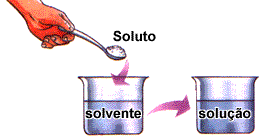
\includegraphics[scale=0.6]{solucao.png}
			\label{}
		\end{figure}
		
		
	\end{frame}


	\section{Quarta Questão}
	\subsection{Cálculo para Computação}
	\begin{frame}
		4) Uma lancha se desloca numa lagoa com a velocidade de 10 m/s. Em dado instante seu motor é desligado; a lancha sofre com isso uma redução de velocidade proporcional à resistência da água. Sabendo-se que ao cabo de 5 s sua velocidade é de 8 m/s, qual será o tempo necessário para que a lancha  adquira velocidade de 1 m/s?
		
		\centering
		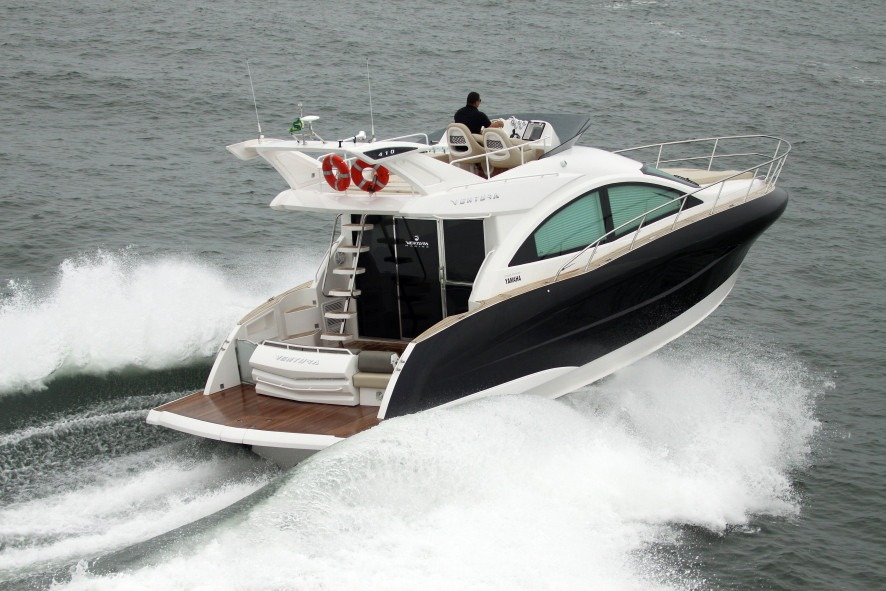
\includegraphics[scale=0.23]{lancha.jpg}
		\label{}
	\end{frame}
	
	\begin{frame}
		\begin{displaymath}
			F = ma \implies m\frac{dv}{dt} = -Kv
		\end{displaymath} \pause
		
		Separando as variáveis:
		
		\begin{displaymath}
			m\int \frac{dv}{v} = \int -K dt \therefore m\ln v = -Kt + C
		\end{displaymath}
		
		Para t = 0 e v = 10 m/s temos que \boxed{ C = 2,3025m }
		Para t = 5, v = 8 m/s: \pause
		
		\begin{displaymath}
			m \ln 8 = - 5K + 2,3025m
		\end{displaymath} \pause
		
		\begin{displaymath}
			m(\ln 8 - 2,3025) = -5K
		\end{displaymath} \pause
		
		\begin{displaymath}
			m(2,0794 - 2,3025) = - 5K
		\end{displaymath} \pause
	
		\begin{equation}
			\boxed{ -0,2231m = - 5K }
		\end{equation}
	\end{frame}

	\begin{frame}
		Quando v = 1 m/s, t = ? 
		
		\begin{displaymath}
			m\ln 1 = -Kt + 2,3025m
		\end{displaymath} \pause
	
		\begin{displaymath}
			m(\ln 1 - 2,3025) = -Kt
		\end{displaymath} \pause	
		
		\begin{equation}
			2,3025m = Kt \therefore \boxed{ m = \frac{Kt}{2,3025} }
		\end{equation} \pause
		
		Substituindo o valor de m na equação (1):
		
		\begin{displaymath}
			0,2231 \frac{Kt}{2,3025} = 5K \therefore t = \frac{5(2,3025)}{0,2231} \therefore \boxed{ t = 51,6 \text{ s} }
		\end{displaymath}
	
	
	
	
	\end{frame}
	
\end{document}